\subsection{Гистограмма и график плотности распределения}
	\begin{figure}[h]
		\center{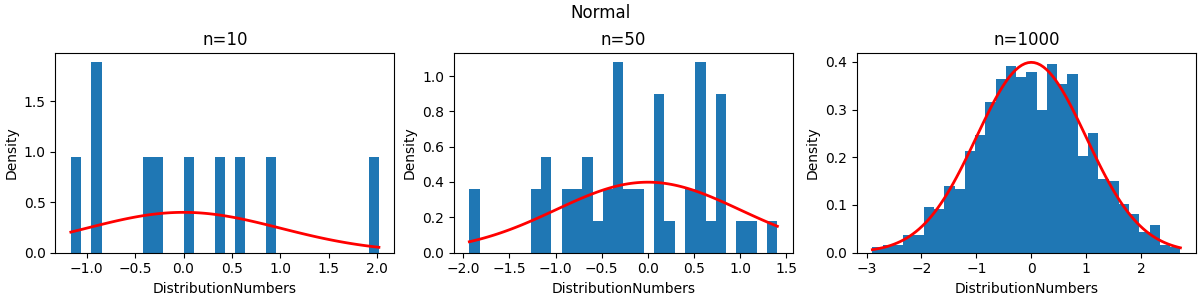
\includegraphics[width=1\linewidth]{DistributionHistograms/Normal.png}}
		\caption{Нормальное распределение}
		\label{ris:image}
	\end{figure}
	
	\begin{figure}[h]
		\center{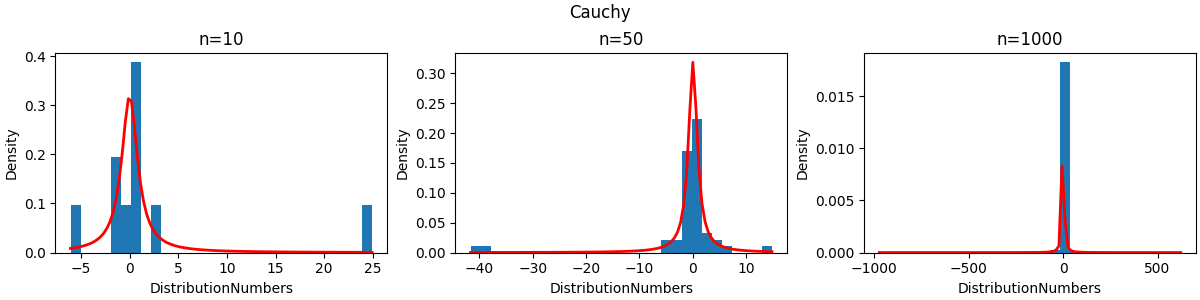
\includegraphics[width=1\linewidth]{DistributionHistograms/Cauchy.png}}
		\caption{Распределение Коши}
		\label{ris:image}
	\end{figure}

	\begin{figure}[h]
		\center{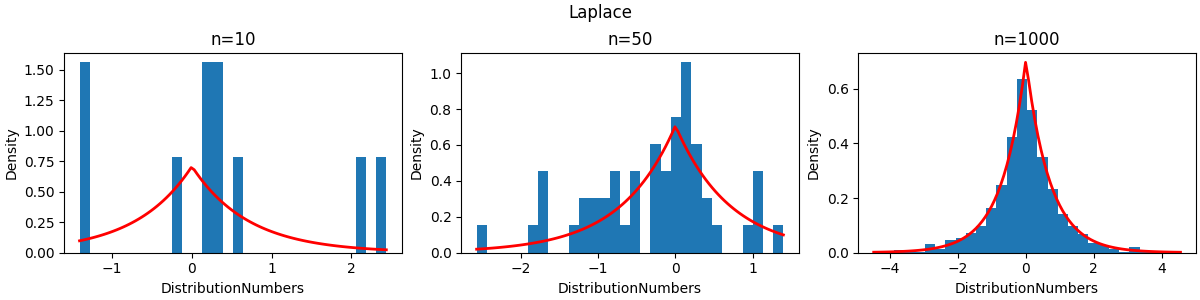
\includegraphics[width=1\linewidth]{DistributionHistograms/Laplace.png}}
		\caption{Распределение Лапласа}
		\label{ris:image}
	\end{figure}

	\begin{figure}[h]
		\center{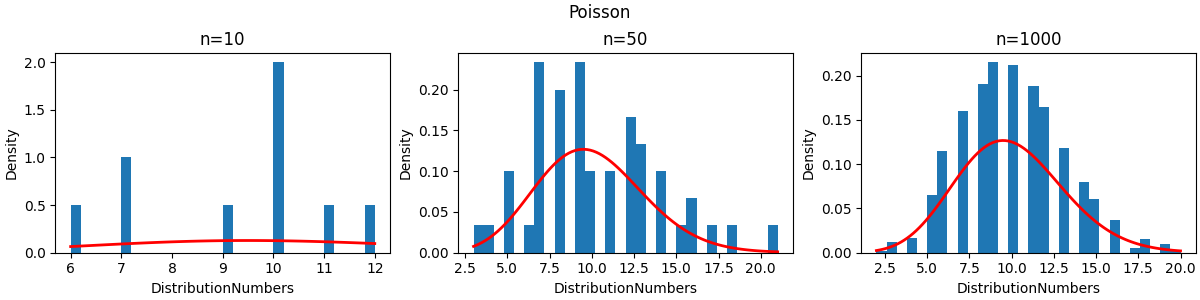
\includegraphics[width=1\linewidth]{DistributionHistograms/Poisson.png}}
		\caption{Распределение Пуассона}
		\label{ris:image}
	\end{figure}

	\begin{figure}[h]
		\center{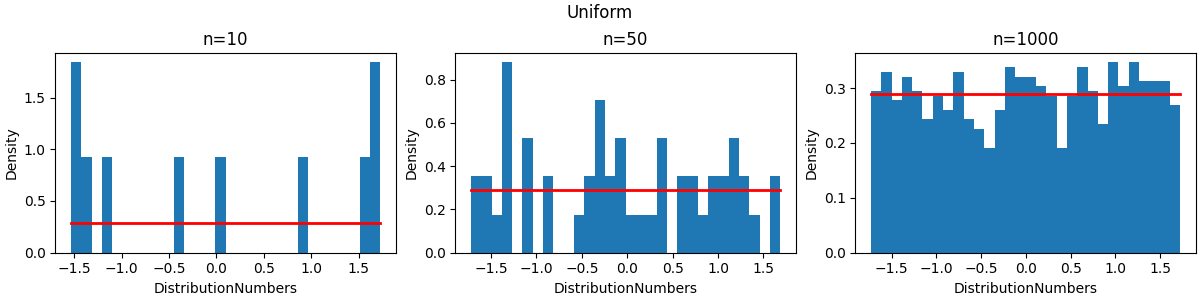
\includegraphics[width=1\linewidth]{DistributionHistograms/Uniform.png}}
		\caption{Равномерное распределение}
		\label{ris:image}
	\end{figure}

\subsection{Характеристики положения и рассеяния}
	\begin{table}[H]
		\label{tabular:timesandtenses}
		\begin{center}
			\begin{tabular}{|c | c | c | c | c | c|} 
 \hline \multicolumn{6}{|c|}{normal} \\ 
 \hline & $\bar{x}$ & $medx$ & $z_R$ & $z_Q$ & $z_{tr}$ 
 \\ \hline $n=10$ & & & & & \\ 
 \hline $E(z)$ 
 &0.008238 &0.248319 &-0.015972 &0.010999 &-0.090915 \\ 
 \hline $D(z)$ 
 &0.092668 &0.1526 &0.182401 &0.117243 &0.078463 \\ 
\hline $\hat{E}(z)$ 
&0.0&0.0&-0.0&0.0&-0.1 \\ 
\hline $E-\sqrt{D(z)}$ 
&-0.296176&-0.142321&-0.443057&-0.331408&-0.371027 \\ 
\hline $E+\sqrt{D(z)}$ 
&0.312652&0.638959&0.411112&0.353407&0.189197 \\ \hline $n=100$ & & & & & \\ 
 \hline $E(z)$ 
 &0.001544 &0.029189 &-0.009478 &-0.000188 &-0.009312 \\ 
 \hline $D(z)$ 
 &0.011024 &0.015996 &0.090679 &0.012835 &0.011323 \\ 
\hline $\hat{E}(z)$ 
&0.0&0.0&-0.0&-0.0&-0.0 \\ 
\hline $E-\sqrt{D(z)}$ 
&-0.103451&-0.097286&-0.310608&-0.113479&-0.115722 \\ 
\hline $E+\sqrt{D(z)}$ 
&0.106539&0.155664&0.291652&0.113104&0.097098 \\ \hline $n=1000$ & & & & & \\ 
 \hline $E(z)$ 
 &0.000919 &0.001296 &-0.001158 &0.001068 &-0.001927 \\ 
 \hline $D(z)$ 
 &0.001006 &0.001525 &0.061366 &0.001207 &0.001232 \\ 
\hline $\hat{E}(z)$ 
&0.0&0.0&-0.0&0.0&-0.0 \\ 
\hline $E-\sqrt{D(z)}$ 
&-0.030799&-0.037755&-0.248879&-0.033675&-0.037022 \\ 
\hline $E+\sqrt{D(z)}$ 
&0.032638&0.040347&0.246563&0.035812&0.033169 \\ \hline 
 \end{tabular}
		\end{center}
		\caption{Нормальное распределение}
	\end{table}
	
	\begin{table}[H]
		\label{tabular:timesandtenses}
		\begin{center}
			\begin{tabular}{|c | c | c | c | c | c|} 
 \hline \multicolumn{6}{|c|}{cauchy} \\ 
 \hline & $\bar{x}$ & $medx$ & $z_R$ & $z_Q$ & $z_{tr}$ 
 \\ \hline $n=10$ & & & & & \\ 
 \hline $E(z)$ 
 &1.818012 &0.396859 &1.447601 &0.012234 &-0.212547 \\ 
 \hline $D(z)$ 
 &3556.173955 &0.492939 &56281.61374 &0.970573 &0.292936 \\ 
\hline $\hat{E}(z)$ 
&2.0&0.0&1.0&0.0&-0.0 \\ 
\hline $E-\sqrt{D(z)}$ 
&-57.815653&-0.305237&-235.789862&-0.972942&-0.753783 \\ 
\hline $E+\sqrt{D(z)}$ 
&61.451677&1.098955&238.685064&0.997411&0.328689 \\ \hline $n=100$ & & & & & \\ 
 \hline $E(z)$ 
 &3.147533 &0.034373 &-0.071036 &-0.004734 &-0.013174 \\ 
 \hline $D(z)$ 
 &8029.837854 &0.027524 &923012.911793 &0.053112 &0.024438 \\ 
\hline $\hat{E}(z)$ 
&3.0&0.0&-0.0&-0.0&-0.0 \\ 
\hline $E-\sqrt{D(z)}$ 
&-86.461829&-0.131531&-960.806646&-0.235196&-0.1695 \\ 
\hline $E+\sqrt{D(z)}$ 
&92.756896&0.200277&960.664574&0.225727&0.143153 \\ \hline $n=1000$ & & & & & \\ 
 \hline $E(z)$ 
 &-0.438253 &0.003758 &99.544606 &-0.001103 &-0.000183 \\ 
 \hline $D(z)$ 
 &759.178592 &0.002403 &254576161.398767 &0.004782 &0.00234 \\ 
\hline $\hat{E}(z)$ 
&-0.0&0.0&100.0&-0.0&-0.0 \\ 
\hline $E-\sqrt{D(z)}$ 
&-27.991449&-0.045258&-15855.898396&-0.070253&-0.048556 \\ 
\hline $E+\sqrt{D(z)}$ 
&27.114942&0.052774&16054.987609&0.068048&0.048191 \\ \hline 
 \end{tabular}
		\end{center}
		\caption{Распределение Коши}
	\end{table}

	\begin{table}[H]
		\label{tabular:timesandtenses}
		\begin{center}
			\begin{tabular}{|c | c | c | c | c | c|} 
 \hline \multicolumn{6}{|c|}{laplace} \\ 
 \hline & $\bar{x}$ & $medx$ & $z_R$ & $z_Q$ & $z_{tr}$ 
 \\ \hline $n=10$ & & & & & \\ 
 \hline $E(z)$ 
 &-0.012064 &0.167808 &-0.015735 &0.003608 &-0.077328 \\ 
 \hline $D(z)$ 
 &0.098635 &0.078996 &0.450001 &0.093068 &0.050183 \\ 
\hline $\hat{E}(z)$ 
&-0.0&0.2&-0.0&0.0&-0.1 \\ 
\hline $E-\sqrt{D(z)}$ 
&-0.326126&-0.113253&-0.686556&-0.301463&-0.301345 \\ 
\hline $E+\sqrt{D(z)}$ 
&0.301998&0.44887&0.655086&0.308678&0.146688 \\ \hline $n=100$ & & & & & \\ 
 \hline $E(z)$ 
 &0.000819 &0.015549 &0.028057 &0.002266 &-0.017529 \\ 
 \hline $D(z)$ 
 &0.010053 &0.006059 &0.393641 &0.010114 &0.006032 \\ 
\hline $\hat{E}(z)$ 
&0.0&0.0&0.0&0.0&-0.0 \\ 
\hline $E-\sqrt{D(z)}$ 
&-0.099443&-0.062288&-0.599351&-0.098302&-0.095195 \\ 
\hline $E+\sqrt{D(z)}$ 
&0.101082&0.093386&0.655465&0.102834&0.060136 \\ \hline $n=1000$ & & & & & \\ 
 \hline $E(z)$ 
 &-0.000927 &0.002156 &0.010106 &2.5e-05 &-0.000258 \\ 
 \hline $D(z)$ 
 &0.001001 &0.000528 &0.38354 &0.001005 &0.000649 \\ 
\hline $\hat{E}(z)$ 
&-0.0&0.0&0.0&0.0&-0.0 \\ 
\hline $E-\sqrt{D(z)}$ 
&-0.03257&-0.02083&-0.6092&-0.031678&-0.025737 \\ 
\hline $E+\sqrt{D(z)}$ 
&0.030715&0.025141&0.629412&0.031729&0.025221 \\ \hline 
 \end{tabular}
		\end{center}
		\caption{Распределение Лапласа}
	\end{table}

	\begin{table}[H]
		\label{tabular:timesandtenses}
		\begin{center}
			\begin{tabular}{|c | c | c | c | c | c|} 
 \hline \multicolumn{6}{|c|}{poisson} \\ 
 \hline & $\bar{x}$ & $medx$ & $z_R$ & $z_Q$ & $z_{tr}$ 
 \\ \hline $n=10$ & & & & & \\ 
 \hline $E(z)$ 
 &10.0418 &10.6325 &10.3215 &9.8945 &7.879167 \\ 
 \hline $D(z)$ 
 &0.997813 &1.471194 &1.945888 &1.10462 &0.804316 \\ 
\hline $\hat{E}(z)$ 
&10.0&11.0&10.0&10.0&8.0 \\ 
\hline $E-\sqrt{D(z)}$ 
&9.042894&9.419572&8.926549&8.843491&6.98233 \\ 
\hline $E+\sqrt{D(z)}$ 
&11.040706&11.845428&11.716451&10.945509&8.776003 \\ \hline $n=100$ & & & & & \\ 
 \hline $E(z)$ 
 &10.00482 &9.922 &10.9225 &9.9155 &9.63366 \\ 
 \hline $D(z)$ 
 &0.096424 &0.218916 &0.994744 &0.13936 &0.120093 \\ 
\hline $\hat{E}(z)$ 
&10.0&10.0&11.0&10.0&10.0 \\ 
\hline $E-\sqrt{D(z)}$ 
&9.694299&9.454115&9.925132&9.542191&9.287116 \\ 
\hline $E+\sqrt{D(z)}$ 
&10.315341&10.389885&11.919868&10.288809&9.980204 \\ \hline $n=1000$ & & & & & \\ 
 \hline $E(z)$ 
 &9.998306 &9.997 &11.677 &9.993375 &9.83299 \\ 
 \hline $D(z)$ 
 &0.009314 &0.002991 &0.655671 &0.003222 &0.010328 \\ 
\hline $\hat{E}(z)$ 
&10.0&10.0&12.0&10.0&9.8 \\ 
\hline $E-\sqrt{D(z)}$ 
&9.901795&9.94231&10.867265&9.936615&9.731365 \\ 
\hline $E+\sqrt{D(z)}$ 
&10.094817&10.05169&12.486735&10.050135&9.934615 \\ \hline 
 \end{tabular}
		\end{center}
		\caption{Распределение Пуассона}
	\end{table}

	\begin{table}[H]
		\label{tabular:timesandtenses}
		\begin{center}
			\begin{tabular}{|c | c | c | c | c | c|} 
 \hline \multicolumn{6}{|c|}{uniform} \\ 
 \hline & $\bar{x}$ & $medx$ & $z_R$ & $z_Q$ & $z_{tr}$ 
 \\ \hline $n=10$ & & & & & \\ 
 \hline $E(z)$ 
 &-0.008418 &0.293364 &0.010974 &-0.011414 &-0.130199 \\ 
 \hline $D(z)$ 
 &0.100766 &0.21381 &0.044133 &0.136721 &0.125672 \\ 
\hline $\hat{E}(z)$ 
&-0.0&0.0&0.0&-0.0&-0.0 \\ 
\hline $E-\sqrt{D(z)}$ 
&-0.325855&-0.169032&-0.199104&-0.381173&-0.484701 \\ 
\hline $E+\sqrt{D(z)}$ 
&0.309019&0.75576&0.221053&0.358345&0.224303 \\ \hline $n=100$ & & & & & \\ 
 \hline $E(z)$ 
 &0.000993 &0.03263 &-0.00032 &-0.000481 &-0.009553 \\ 
 \hline $D(z)$ 
 &0.009658 &0.030279 &0.000614 &0.015005 &0.019282 \\ 
\hline $\hat{E}(z)$ 
&0.0&0.0&-0.0&-0.0&-0.0 \\ 
\hline $E-\sqrt{D(z)}$ 
&-0.097283&-0.141379&-0.025097&-0.122976&-0.148414 \\ 
\hline $E+\sqrt{D(z)}$ 
&0.099268&0.20664&0.024458&0.122015&0.129308 \\ \hline $n=1000$ & & & & & \\ 
 \hline $E(z)$ 
 &-0.000426 &0.004564 &-0.000143 &-0.000327 &-0.004165 \\ 
 \hline $D(z)$ 
 &0.001026 &0.002894 &6e-06 &0.001484 &0.002194 \\ 
\hline $\hat{E}(z)$ 
&-0.0&0.0&-0.0&-0.0&-0.0 \\ 
\hline $E-\sqrt{D(z)}$ 
&-0.032461&-0.049232&-0.00257&-0.038851&-0.051007 \\ 
\hline $E+\sqrt{D(z)}$ 
&0.031608&0.058361&0.002283&0.038197&0.042677 \\ \hline 
 \end{tabular}
		\end{center}
		\caption{Равномерное распределение}
	\end{table}

\subsection{Боксплот Тьюки}
	\begin{figure}[H]
		\center{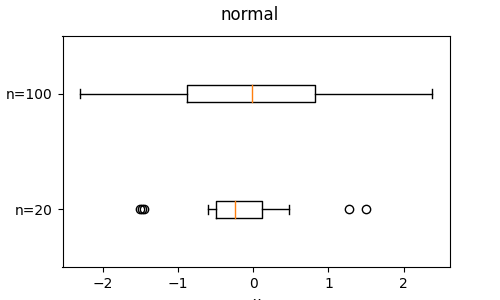
\includegraphics{BoxPlots/normalBoxplot.png}}
		\caption{Нормальное распределение}
		\label{ris:image}
	\end{figure}

	\begin{figure}[H]
		\center{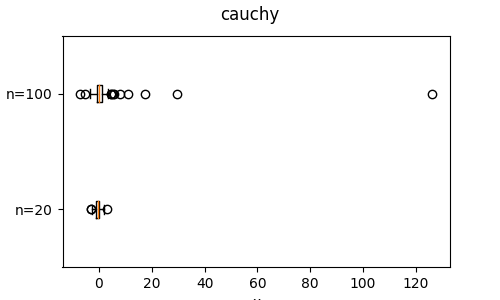
\includegraphics{BoxPlots/cauchyBoxplot.png}}
		\caption{Распределение Коши}
		\label{ris:image}
	\end{figure}

	\begin{figure}[H]
		\center{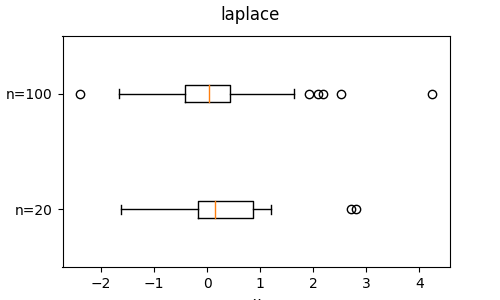
\includegraphics{BoxPlots/laplaceBoxplot.png}}
		\caption{Распределение Лапласа}
		\label{ris:image}
	\end{figure}

	\begin{figure}[H]
		\center{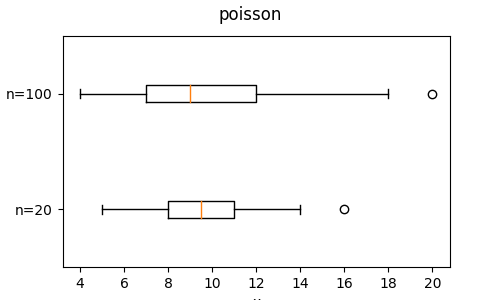
\includegraphics{BoxPlots/poissonBoxplot.png}}
		\caption{Распределение Пуассона}
		\label{ris:image}
	\end{figure}

	\begin{figure}[H]
		\center{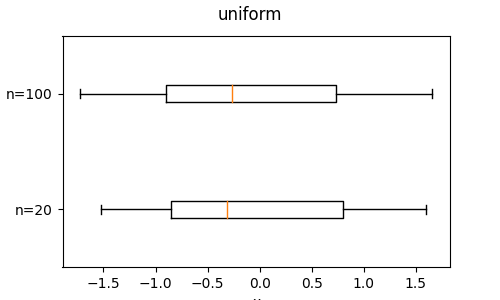
\includegraphics{BoxPlots/uniformBoxplot.png}}
		\caption{Равномерное распределение}
		\label{ris:image}
	\end{figure}

\subsection{Доля выбросов}
	\begin{table}[H]
		\label{tabular:timesandtenses}
		\begin{center}
			\begin{tabular}{| c | c |} \hline Sample & Share of emissions \\ \hline normal n = 20 & 0.02 \\ \hline 
 normal n = 100 & 0.01 \\ \hline 
 cauchy n = 20 & 0.15 \\ \hline 
 cauchy n = 100 & 0.15 \\ \hline 
 laplace n = 20 & 0.07 \\ \hline 
 laplace n = 100 & 0.06 \\ \hline 
 poisson n = 20 & 0.03 \\ \hline 
 poisson n = 100 & 0.01 \\ \hline 
 uniform n = 20 & 0.0 \\ \hline 
 uniform n = 100 & 0.0 \\ \hline 
 \end{tabular}
		\end{center}
		\caption{Нормальное распределение}
	\end{table}

\subsection{Теоретическая вероятность выбросов}
	\begin{table}[H]
		\label{tabular:timesandtenses}
		\begin{center}
			\begin{tabular}{| c | c |} \hline Распределение & $P_B^T (17) (18)$ \\ \hline
				 Нормальное распределение & 0.007 \\ \hline 
				 Распределение Коши & 0.156 \\ \hline 
				 Распределение Лапласа& 0.063 \\ \hline 
				 Распределение Пуассона & 0.008 \\ \hline 
				 Равномерное распределение & 0 \\ \hline 
			 \end{tabular}
		\end{center}
		\caption{Нормальное распределение}
	\end{table}

\subsection{Эмпирическая функция распределения}
	\begin{figure}[H]
		\center{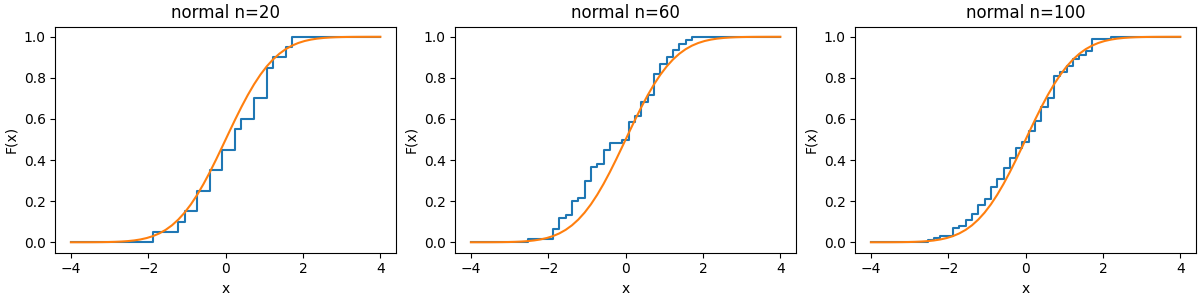
\includegraphics[width=1\linewidth]{empirical_distribution/cdfnormal.png}}
		\caption{Нормальное распределение}
		\label{ris:image}
	\end{figure}

	\begin{figure}[H]
		\center{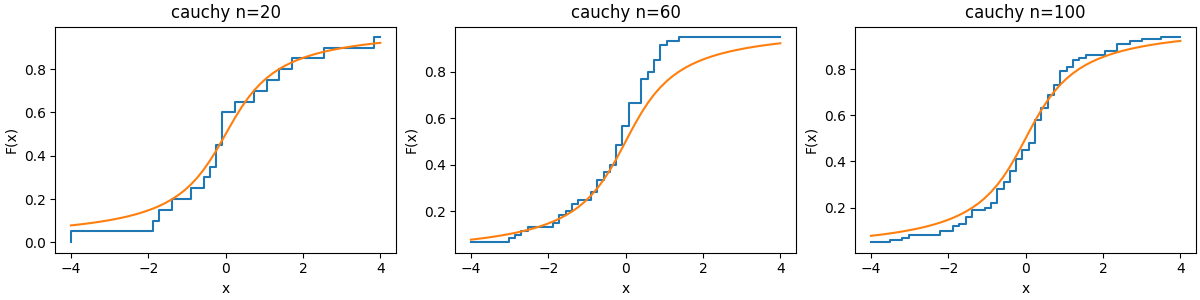
\includegraphics[width=1\linewidth]{empirical_distribution/cdfcauchy.png}}
		\caption{Распределение Коши}
		\label{ris:image}
	\end{figure}

	\begin{figure}[H]
		\center{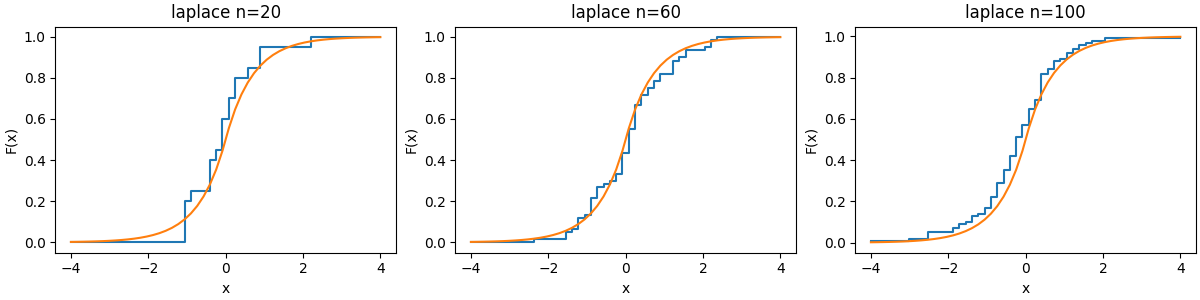
\includegraphics[width=1\linewidth]{empirical_distribution/cdflaplace.png}}
		\caption{Распределение Лапласа}
		\label{ris:image}
	\end{figure}

	\begin{figure}[H]
		\center{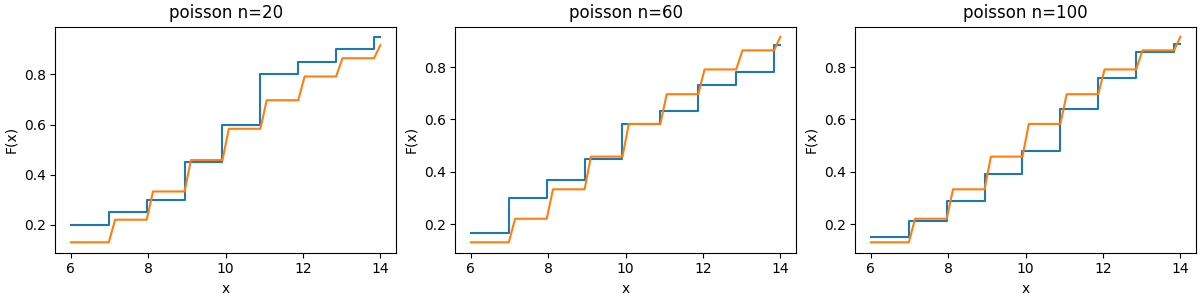
\includegraphics[width=1\linewidth]{empirical_distribution/cdfpoisson.png}}
		\caption{Распределение Пуассона}
		\label{ris:image}
	\end{figure}

	\begin{figure}[H]
		\center{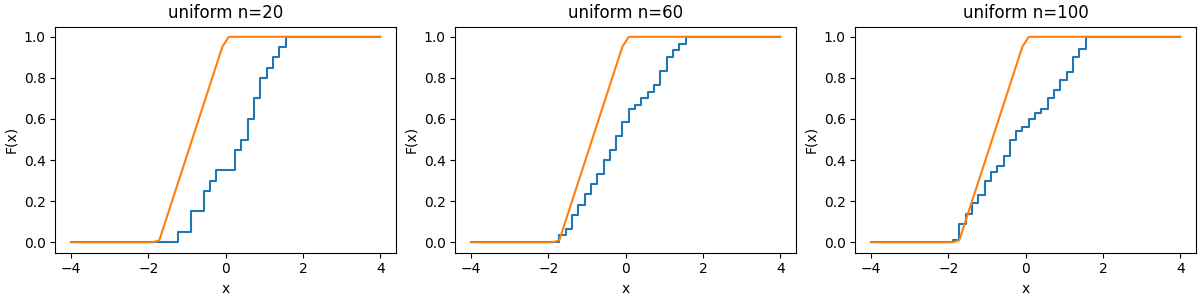
\includegraphics[width=1\linewidth]{empirical_distribution/cdfuniform.png}}
		\caption{Равномерное распределение}
		\label{ris:image}
	\end{figure}

\subsection{Ядерные оценки плотности распределения}
	\begin{figure}[H]
		\center{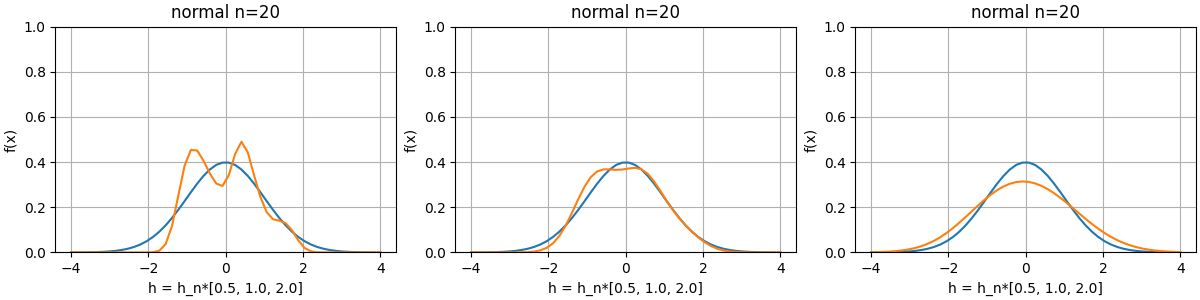
\includegraphics[width=1\linewidth]{KDE/kdeN=20 normal.png}}
		\caption{Нормальное распределение, n = 20}
		\label{ris:image}
	\end{figure}
	
	\begin{figure}[H]
		\center{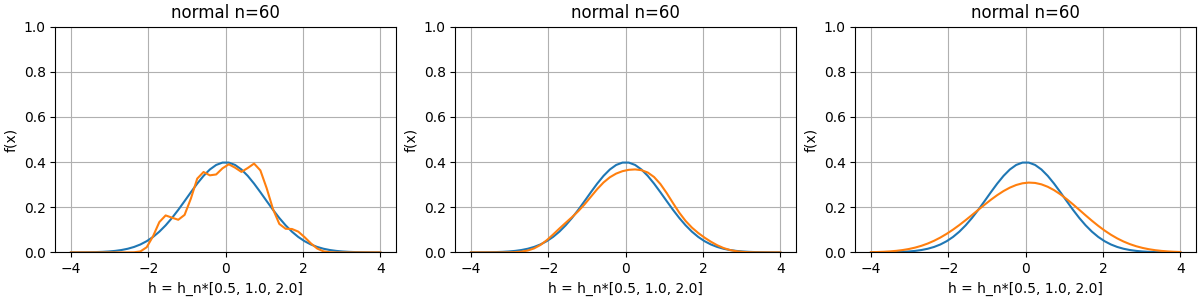
\includegraphics[width=1\linewidth]{KDE/kdeN=60 normal.png}}
		\caption{Нормальное распределение, n = 60}
		\label{ris:image}
	\end{figure}

	\begin{figure}[H]
		\center{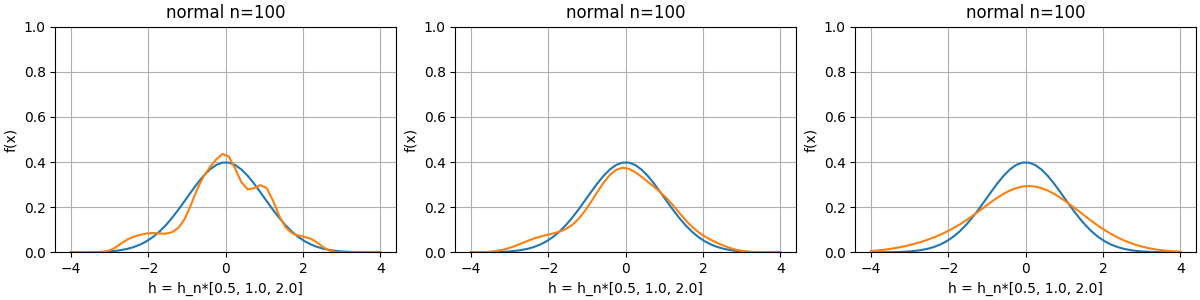
\includegraphics[width=1\linewidth]{KDE/kdeN=100 normal.png}}
		\caption{Нормальное аспределение, n = 100}
		\label{ris:image}
	\end{figure}

	\begin{figure}[H]
		\center{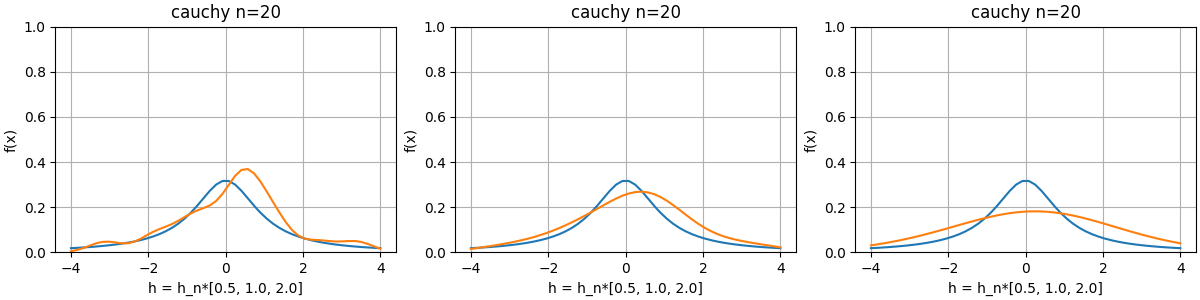
\includegraphics[width=1\linewidth]{KDE/kdeN=20 cauchy.png}}
		\caption{Распределение Коши, n = 20}
		\label{ris:image}
	\end{figure}
	
	\begin{figure}[H]
		\center{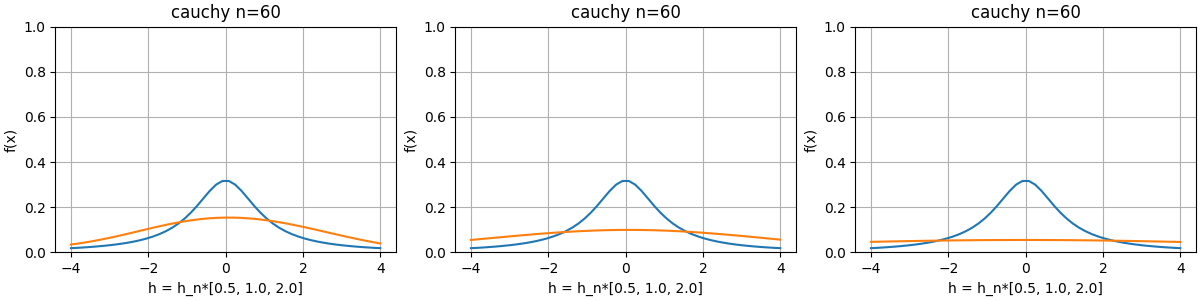
\includegraphics[width=1\linewidth]{KDE/kdeN=60 cauchy.png}}
		\caption{Распределение Коши, n = 60}
		\label{ris:image}
	\end{figure}

	\begin{figure}[H]
		\center{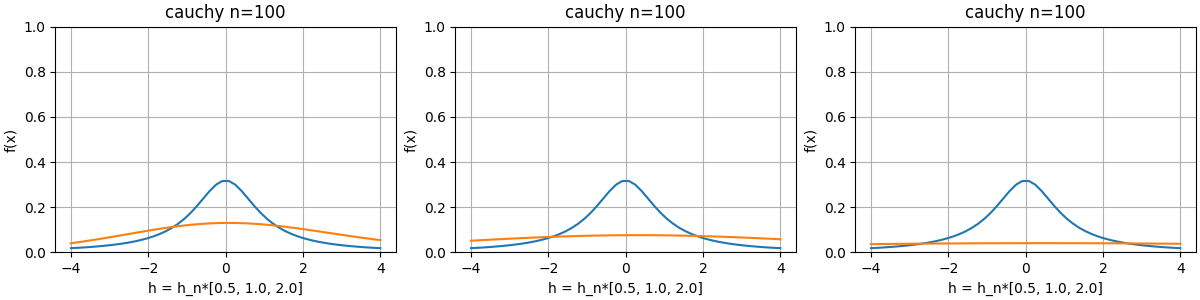
\includegraphics[width=1\linewidth]{KDE/kdeN=100 cauchy.png}}
		\caption{Распределение Коши, n = 100}
		\label{ris:image}
	\end{figure}
	
	\begin{figure}[H]
		\center{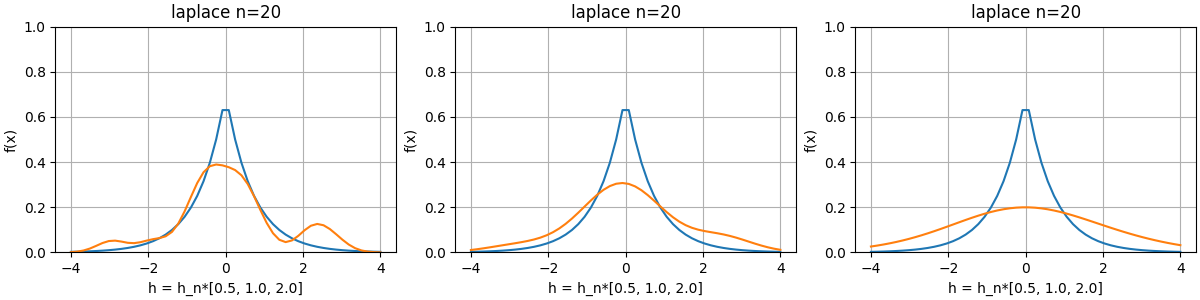
\includegraphics[width=1\linewidth]{KDE/kdeN=20 laplace.png}}
		\caption{Распределение Лапласа, n = 20}
		\label{ris:image}
	\end{figure}
	
	\begin{figure}[H]
		\center{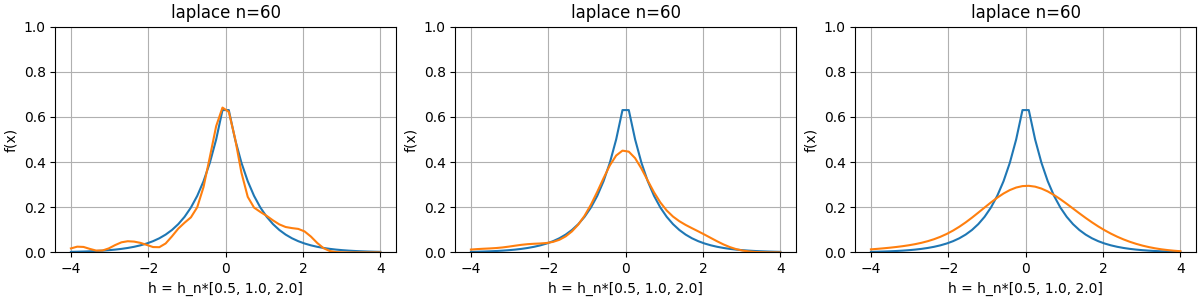
\includegraphics[width=1\linewidth]{KDE/kdeN=60 laplace.png}}
		\caption{Распределение Лапласа, n = 60}
		\label{ris:image}
	\end{figure}

	\begin{figure}[H]
		\center{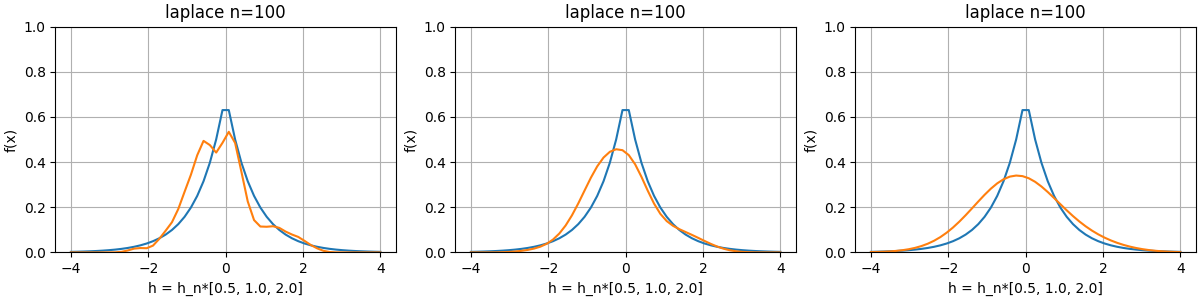
\includegraphics[width=1\linewidth]{KDE/kdeN=100 laplace.png}}
		\caption{Распределение Лапласа, n = 100}
		\label{ris:image}
	\end{figure}
	
	\begin{figure}[H]
		\center{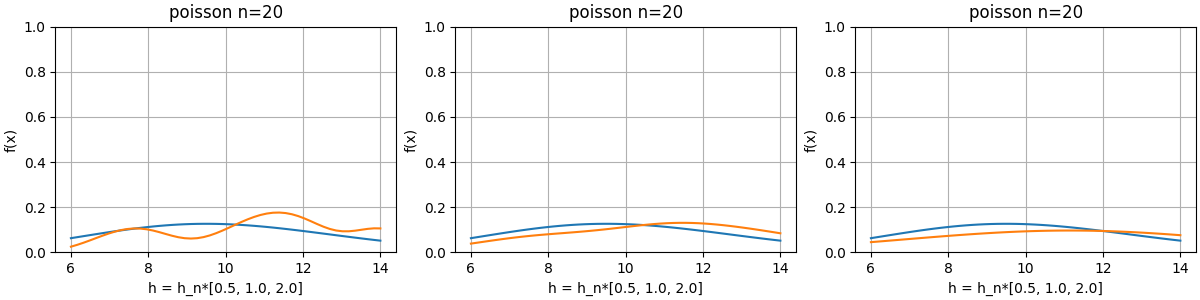
\includegraphics[width=1\linewidth]{KDE/kdeN=20 poisson.png}}
		\caption{Распределение Пуассона, n = 20}
		\label{ris:image}
	\end{figure}
	
	\begin{figure}[H]
		\center{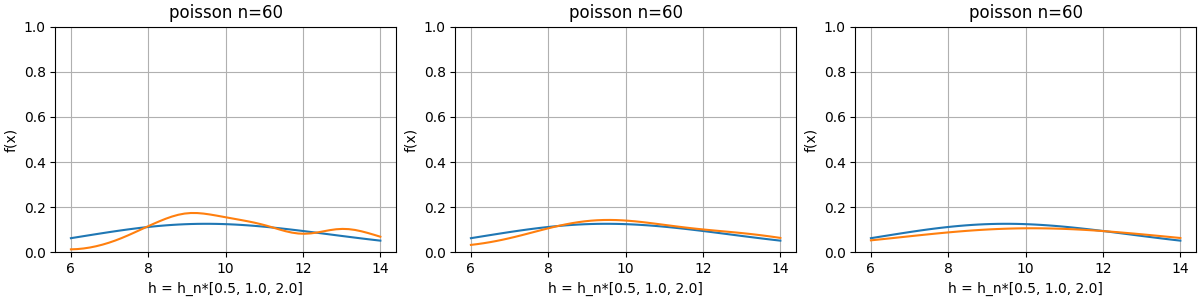
\includegraphics[width=1\linewidth]{KDE/kdeN=60 poisson.png}}
		\caption{Распределение Пуассона, n = 60}
		\label{ris:image}
	\end{figure}

	\begin{figure}[H]
		\center{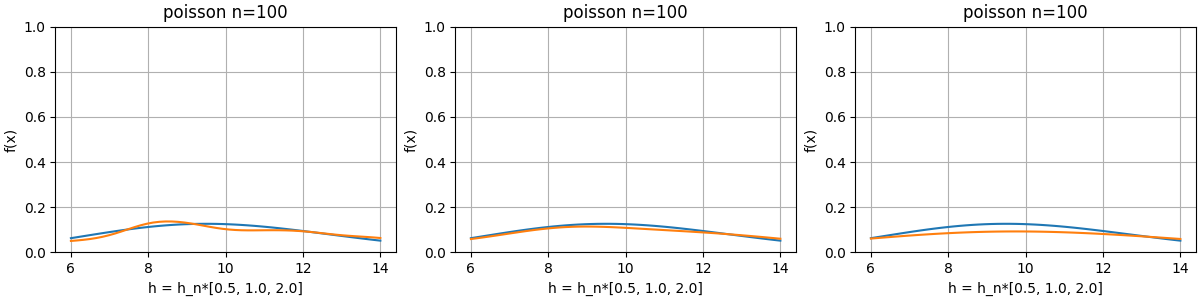
\includegraphics[width=1\linewidth]{KDE/kdeN=100 poisson.png}}
		\caption{Распределение Пуассона, n = 100}
		\label{ris:image}
	\end{figure}
	%
	\begin{figure}[H]
		\center{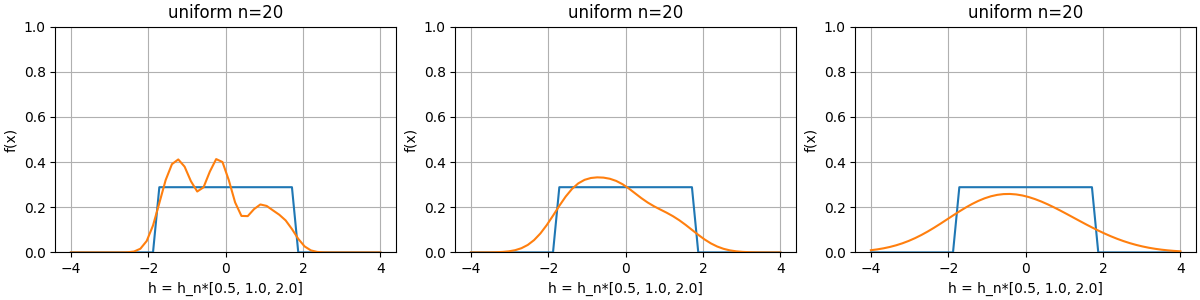
\includegraphics[width=1\linewidth]{KDE/kdeN=20 uniform.png}}
		\caption{Равномерное распределение, n = 20}
		\label{ris:image}
	\end{figure}
	
	\begin{figure}[H]
		\center{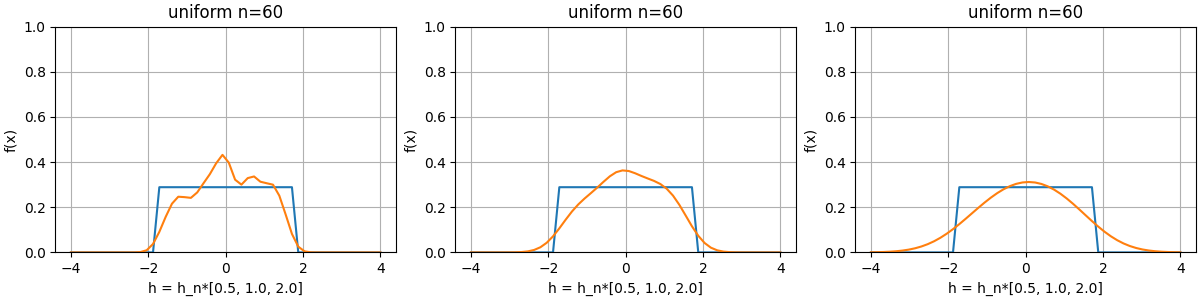
\includegraphics[width=1\linewidth]{KDE/kdeN=60 uniform.png}}
		\caption{Равномерное распределение, n = 60}
		\label{ris:image}
	\end{figure}

	\begin{figure}[H]
		\center{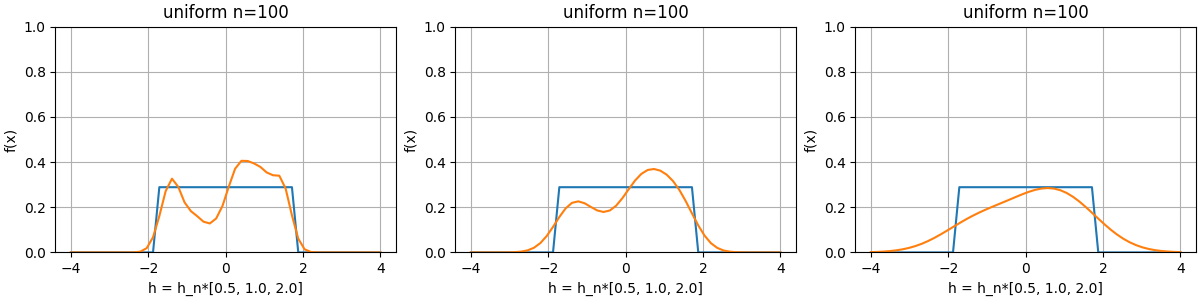
\includegraphics[width=1\linewidth]{KDE/kdeN=100 uniform.png}}
		\caption{Равномерное распределение, n = 100}
		\label{ris:image}
	\end{figure}

